\documentclass[11pt,a4paper]{article}

% ---------- Paquets ----------
\usepackage[utf8]{inputenc}
\usepackage[T1]{fontenc}
\usepackage[french]{babel}
\usepackage{lmodern}
\usepackage[margin=2.5cm]{geometry}
\usepackage{amsmath,amssymb}
\usepackage{icomma}
\usepackage{graphicx}
\usepackage{float}
\usepackage{caption}
\usepackage{subcaption}
\usepackage{array}
\usepackage{xcolor}
\usepackage{xspace}
\usepackage{pgfplots}
\pgfplotsset{compat=1.18}
\usetikzlibrary{babel}
\usepackage[hidelinks]{hyperref}

\definecolor{orangeesir}{RGB}{230,120,40}
\pgfplotsset{/pgf/number format/.cd, use comma, 1000 sep={\,}}
\graphicspath{{images/}}
\renewcommand{\arraystretch}{1.2}
\newcommand{\us}{\,\textmu s\xspace}

\begin{document}

% =====================================================================
%                          PAGE DE GARDE
% =====================================================================
\pagenumbering{gobble}
\begin{titlepage}
\begin{tikzpicture}[remember picture,overlay]
  \draw[line width=0.6pt]
    ([xshift=2cm,yshift=-2cm]current page.north west)
    rectangle
    ([xshift=-2cm,yshift=2cm]current page.south east);
\end{tikzpicture}

\centering
\vspace*{0.3cm}


\includegraphics[width=0.45\textwidth]{logo_univ_rennes.png}

\vspace{1cm}


\includegraphics[width=0.22\textwidth]{logo esir.png}

\vspace{3cm}

{\Large\bfseries \underline{Travaux Pratiques 2 :} Transformée de Fourier rapide\par}
\vspace{0.3cm}
{\large FFT récursive, multiplication de polynômes,\\ analyse fréquentielle et compression d'images\par}
\vspace{0.3cm}
Algorithmique et Complexité, ESIR 2 IOT

\vspace{3cm}

\begin{minipage}[t]{0.42\textwidth}
  \centering
  {\color{orangeesir}\bfseries PROFESSEUR}\\[0.3cm]
  \fbox{\parbox[c][2cm][c]{0.9\linewidth}{\centering M. Pierre MAUREL}}
\end{minipage}
\hfill
\begin{minipage}[t]{0.42\textwidth}
  \centering
  {\color{orangeesir}\bfseries ÉTUDIANTS}\\[0.3cm]
  \fbox{\parbox[c][2cm][c]{0.9\linewidth}{\centering
    COULIBALY Yaplé Assétou\\[0.2cm]
    KOUAKOU Yah Mardochée}}
\end{minipage}

\vfill

\fbox{\parbox{0.6\textwidth}{\centering\bfseries\itshape ANNÉE ACADÉMIQUE : 2026-2027}}

\vspace{0.5cm}
\end{titlepage}

\pagenumbering{roman}
\tableofcontents
\newpage
\pagenumbering{arabic}

% =====================================================================

% =====================================================================
\section{Objectifs du TP}
% =====================================================================

Le TP a deux parties. Dans la première, on programme une FFT récursive et son
inverse, on s'en sert pour multiplier des polynômes et on compare les temps de
calcul avec la multiplication par les coefficients, pour retrouver
$\Theta(n \log n)$ et $\Theta(n^2)$. Dans la deuxième, on utilise cette FFT pour
analyser des signaux : en 1D d'abord, puis sur des images avec la TFD 2D, et on
l'applique à la compression d'images avec deux méthodes, le carré de basses
fréquences et le seuillage. Pour chaque expérience de la deuxième partie, on a écrit
ce qu'on s'attendait à obtenir avant de lancer le calcul.

\part{FFT et multiplication de polynômes}

\section{FFT récursive et TFD inverse}
% =====================================================================

\subsection{Ce qu'on a fait}

La fonction de combinaison applique les formules de l'énoncé : à partir des TFD des
coefficients pairs et impairs (taille $n/2$), elle calcule les $n$ valeurs
$A(\omega_n^k)$ et $A(\omega_n^{k+n/2})$, avec le même produit
$\omega_n^k A_{\text{impair}}(\omega_{n/2}^k)$ pour les deux. La FFT sépare le vecteur
en indices pairs et impairs, s'appelle sur chaque moitié et combine. On s'arrête à
$n = 1$, où la TFD est le vecteur lui-même ; $n$ doit donc être une puissance de 2.
Pour l'inverse, on a utilisé la formule de l'énoncé : conjuguer, appliquer la FFT,
conjuguer et diviser par $n$.

\subsection{Complexité}

Chaque appel fait deux appels sur $n/2$ et une combinaison en $\Theta(n)$ :
$T(n) = 2\,T(n/2) + \Theta(n)$, donc $T(n) = \Theta(n \log n)$ ($\log_2 n$ niveaux
qui coûtent chacun $\Theta(n)$). L'inverse ajoute deux conjugaisons et une division
en $\Theta(n)$, elle reste en $\Theta(n \log n)$. Notre version crée deux tableaux et
calcule un cosinus et un sinus à chaque appel : ça ne change pas la complexité, mais
ça augmente la constante, ce qu'on retrouve dans les mesures.

\subsection{Tests}

Sur l'exemple du TD, $a = (1, 2, 3, 4)$, on attendait
$A(1) = 10$, $A(i) = -2 - 2i$, $A(-1) = -2$, $A(-i) = -2 + 2i$. Notre FFT renvoie
exactement $[\,10,\ -2-2i,\ -2,\ -2+2i\,]$, et l'inverse appliquée à ce résultat
redonne $[\,1,\ 2,\ 3,\ 4\,]$.

% =====================================================================
\section{Multiplication de polynômes}
% =====================================================================

On a suivi la méthode du TD : FFT de $A$ et de $B$, produit terme à terme, FFT
inverse, soit $\Theta(n \log n)$ au total. Le produit est de degré $2n-2$ : il faut
au moins $2n-1$ points, donc on complète les deux vecteurs avec des zéros jusqu'à la
taille $2n$ (qui reste une puissance de 2). On a testé les deux exemples de l'énoncé
et $A_3 \times B_3$ avec $A_3 = 1 + 2X + 3X^2 + 4X^3$ et $B_3 = -3 + 2X - 5X^2$, dont
le produit attendu est $-3 - 4X - 10X^2 - 16X^3 - 7X^4 - 20X^5$.

\begin{table}[H]
\centering
\caption{Tests de la multiplication par FFT.}
\label{tab:mult}
\begin{tabular}{|l|l|l|}
\hline
\textbf{Produit} & \textbf{Résultat attendu} & \textbf{Coefficients obtenus} \\
\hline
$2 \times (-3)$ & $-6$ & $[\,-6,\ 0\,]$ \\
\hline
$(2 + X)(-3 + 2X)$ & $-6 + X + 2X^2$ & $[\,-6,\ 1,\ 2,\ 0\,]$ \\
\hline
$A_3 \times B_3$ & voir ci-dessus &
  $[\,-3,\ -4,\ -10,\ -16,\ -7,\ -20,\ 0,\ 0\,]$ \\
\hline
\end{tabular}
\end{table}

Les résultats sont justes, et la méthode par les coefficients donne la même chose
pour $A_3 \times B_3$. Quelques remarques :
\begin{itemize}
  \item on obtient $2n$ valeurs pour $2n-1$ coefficients : la dernière vient du
        doublement de taille et vaut toujours 0 ;
  \item notre fonction suppose que les deux polynômes ont le même nombre de
        coefficients, on a donc écrit $B_3 = (-3, 2, -5, 0)$ ;
  \item les calculs sont faits en flottants, les coefficients sont justes à des
        erreurs d'arrondi près, trop petites pour apparaître à l'affichage.
\end{itemize}

% =====================================================================
\section{Comparaison des temps de calcul}
% =====================================================================

\subsection{Démarche}

On a mesuré le temps de multiplication de deux polynômes aléatoires avec les deux
méthodes, pour $n = 2^6$ à $2^{15}$, en microsecondes. Avant la série, on fait
20 multiplications non mesurées pour que la machine virtuelle Java ait déjà compilé
le code, et pour chaque taille on garde le minimum de 5 exécutions.

Les modèles viennent de la complexité théorique :
\[
  T_{\text{coeff}}(n) = a\,n^2, \qquad T_{\text{FFT}}(n) = b\,n \ln n .
\]
Pour estimer $a$ et $b$ avec toutes les mesures et pas un seul point, on a calculé
$T(n)/n^2$ et $T(n)/(n \ln n)$ pour chaque taille. On a aussi calculé de combien le
temps est multiplié quand $n$ double : on attend 4 pour $n^2$ et
$2 \ln n / \ln(n/2)$, un peu plus de 2, pour $n \ln n$.

\subsection{Méthode par les coefficients}

\begin{table}[H]
\centering
\caption{Méthode par les coefficients (minimum de 5 exécutions).}
\label{tab:coeff}
\begin{tabular}{|r|r|r|r|}
\hline
$n$ & $T(n)$ (\textmu s) & $T(n)/n^2$ ($10^{-3}$\,\textmu s) & $T(n)/T(n/2)$ \\
\hline
64      & 17           & 4,15 & \\
128     & 70           & 4,27 & 4,12 \\
256     & 289          & 4,41 & 4,13 \\
512     & 1\,180       & 4,50 & 4,08 \\
1\,024  & 4\,822       & 4,60 & 4,09 \\
2\,048  & 18\,733      & 4,47 & 3,88 \\
4\,096  & 71\,680      & 4,27 & 3,83 \\
8\,192  & 276\,822     & 4,12 & 3,86 \\
16\,384 & 976\,377     & 3,64 & 3,53 \\
32\,768 & 3\,913\,325  & 3,64 & 4,01 \\
\hline
\end{tabular}
\end{table}

Le temps est multiplié par 3,5 à 4,1 quand $n$ double (3,95 en moyenne) : c'est bien
une croissance en $n^2$. $T(n)/n^2$ reste entre $4{,}1$ et $4{,}6 \cdot 10^{-3}$\us
jusqu'à $n = 8\,192$, puis descend à $3{,}6\cdot 10^{-3}$\us. Avec
$a = 0{,}0044$\us (valeur des petites tailles), le modèle passait 20\,\% au-dessus des
deux derniers points, on a donc pris
\[
  T_{\text{coeff}}(n) \approx 0{,}004 \cdot n^2 \ \text{\textmu s},
\]
qui reste à moins de 13\,\% de toutes les mesures (figure~\ref{fig:coeff}). On
revient sur la baisse du rapport dans la section~\ref{sec:ecarts}.

\begin{figure}[H]
\centering
\begin{tikzpicture}
\begin{axis}[
  width=0.75\linewidth, height=6.5cm,
  xlabel={Taille $n$}, ylabel={Temps (\textmu s)},
  xmin=0, xmax=34000, ymin=0,
  xtick={0,8192,16384,24576,32768}, scaled x ticks=false,
  grid=major, legend pos=north west,
]
\addplot[only marks, mark=*, blue] coordinates {
  (64,17) (128,70) (256,289) (512,1180) (1024,4822) (2048,18733)
  (4096,71680) (8192,276822) (16384,976377) (32768,3913325)
};
\addlegendentry{Mesures}
\addplot[green!60!black, thick, domain=0:33000, samples=100] {0.004*x^2};
\addlegendentry{$T(n) = 0{,}004\, n^2$}
\end{axis}
\end{tikzpicture}
\caption{Méthode par les coefficients : mesures et modèle quadratique.}
\label{fig:coeff}
\end{figure}

\subsection{Méthode par FFT}

\begin{table}[H]
\centering
\caption{Méthode par FFT (minimum de 5 exécutions).}
\label{tab:fft}
\begin{tabular}{|r|r|r|r|r|}
\hline
$n$ & $T(n)$ (\textmu s) & $T(n)/(n \ln n)$ (\textmu s) & $T(n)/T(n/2)$ & attendu \\
\hline
64      & 107     & 0,402 &      &      \\
128     & 234     & 0,377 & 2,19 & 2,33 \\
256     & 512     & 0,361 & 2,19 & 2,29 \\
512     & 1\,861  & 0,583 & 3,63 & 2,25 \\
1\,024  & 2\,926  & 0,412 & 1,57 & 2,22 \\
2\,048  & 5\,276  & 0,338 & 1,80 & 2,20 \\
4\,096  & 6\,767  & 0,199 & 1,28 & 2,18 \\
8\,192  & 13\,590 & 0,184 & 2,01 & 2,17 \\
16\,384 & 28\,445 & 0,179 & 2,09 & 2,15 \\
32\,768 & 60\,935 & 0,179 & 2,14 & 2,14 \\
\hline
\end{tabular}
\end{table}

Jusqu'à $n = 4\,096$, les mesures sont irrégulières : le rapport tourne autour de 0,4
avec un saut à 0,58, et le temps est multiplié par 3,63, puis 1,57, puis 1,28. Un
facteur 1,28 quand $n$ double est impossible pour un algorithme en $n \ln n$ si le code
ne change pas, donc ces mesures sont faussées (section~\ref{sec:ecarts}). À partir de
$n = 8\,192$, le rapport est stable (0,184 ; 0,179 ; 0,179) et les facteurs sont
proches de ceux attendus. On a pris $b$ dans cette zone :
\[
  T_{\text{FFT}}(n) \approx 0{,}18 \cdot n \ln n \ \text{\textmu s},
\]
à moins de 3\,\% des mesures pour $n \geq 8\,192$ (figure~\ref{fig:fft}).

\begin{figure}[H]
\centering
\begin{tikzpicture}
\begin{axis}[
  width=0.75\linewidth, height=6.5cm,
  xlabel={Taille $n$}, ylabel={Temps (\textmu s)},
  xmin=0, xmax=34000, ymin=0,
  xtick={0,8192,16384,24576,32768}, scaled x ticks=false,
  grid=major, legend pos=north west,
]
\addplot[only marks, mark=*, blue] coordinates {
  (64,107) (128,234) (256,512) (512,1861) (1024,2926) (2048,5276)
  (4096,6767) (8192,13590) (16384,28445) (32768,60935)
};
\addlegendentry{Mesures}
\addplot[orange, thick, domain=64:33000, samples=100] {0.18*x*ln(x)};
\addlegendentry{$T(n) = 0{,}18\, n \ln n$}
\end{axis}
\end{tikzpicture}
\caption{Méthode par FFT : mesures et modèle en $n \ln n$.}
\label{fig:fft}
\end{figure}

\subsection{Points qui s'écartent des modèles}
\label{sec:ecarts}

\begin{itemize}
  \item \textbf{FFT, petites tailles.} Les mesures jusqu'à $n = 4\,096$ sont au-dessus
        du modèle et irrégulières. On pense que c'est la compilation à la volée de
        Java : notre échauffement de 20 multiplications ne suffit sans doute pas pour
        les parties du code qui ne tournent qu'une fois par multiplication
        (conjugaison, produit terme à terme, recopie avec les zéros), et elles sont
        encore lentes au début de la série. On ne s'appuie donc que sur les grandes
        tailles pour estimer $b$.
  \item \textbf{Coefficients, changement de niveau.} $T(n)/n^2$ passe d'environ
        $4{,}4$ à $3{,}6 \cdot 10^{-3}$\us entre $n = 8\,192$ et $n = 16\,384$, alors
        que l'algorithme est le même. Une explication possible
        est un changement de fréquence du processeur (ordinateur portable) pendant la
        série. L'écart reste petit devant la croissance du temps, multiplié par plus de
        200\,000 entre $n = 64$ et $n = 32\,768$.
\end{itemize}

\subsection{Comparaison des deux méthodes}

\begin{figure}[H]
\centering
\begin{tikzpicture}
\begin{loglogaxis}[
  width=0.75\linewidth, height=6.5cm,
  xlabel={Taille $n$}, ylabel={Temps (\textmu s)},
  log basis x=2,
  grid=major, legend pos=north west,
]
\addplot[blue, mark=*] coordinates {
  (64,17) (128,70) (256,289) (512,1180) (1024,4822) (2048,18733)
  (4096,71680) (8192,276822) (16384,976377) (32768,3913325)
};
\addlegendentry{Par les coefficients}
\addplot[orange, mark=square*] coordinates {
  (64,107) (128,234) (256,512) (512,1861) (1024,2926) (2048,5276)
  (4096,6767) (8192,13590) (16384,28445) (32768,60935)
};
\addlegendentry{Par FFT}
\end{loglogaxis}
\end{tikzpicture}
\caption{Comparaison des deux méthodes (échelles logarithmiques : $n^2$ donne une
droite de pente 2, $n \ln n$ une pente un peu supérieure à 1).}
\label{fig:comparaison}
\end{figure}

Pour les petites tailles, la FFT est plus lente : 107\us contre 17\us à $n = 64$. Les
courbes se croisent entre $n = 512$ (1\,180\us contre 1\,861\us) et $n = 1\,024$
(4\,822\us contre 2\,926\us). C'est la constante : $b/a \approx 45$, à cause de la
récursion, des tableaux créés et des cosinus et sinus à chaque appel.

Avec les modèles, le croisement est là où $a\,n^2 = b\,n \ln n$, soit
$n / \ln n = b/a \approx 45$, ce qui donne $n \approx 250$. Nos mesures donnent un
croisement plus tard, entre 512 et 1\,024, parce que les temps de la FFT aux petites
tailles sont au-dessus du modèle (section~\ref{sec:ecarts}).

Ensuite l'écart grandit comme $n / \ln n$ : à $n = 32\,768$, la FFT est 64 fois plus
rapide (61\,ms contre 3,9\,s).

\subsection{Extrapolation}

En prolongeant nos deux modèles jusqu'à $n = 2^{20}$ (environ un million de
coefficients) :
\[
  T_{\text{coeff}}(2^{20}) \approx 0{,}004 \times (2^{20})^2\ \text{\textmu s} \approx 73\ \text{min},
  \qquad
  T_{\text{FFT}}(2^{20}) \approx 0{,}18 \times 2^{20} \times \ln(2^{20})\ \text{\textmu s} \approx 2{,}6\ \text{s}.
\]
La FFT serait environ 1\,700 fois plus rapide. Ce sont des extrapolations de nos
modèles, pas des temps théoriques, et elles supposent
que $a$ et $b$ ne changent pas jusqu'à 32 fois notre plus grande taille (par exemple, les données ne tiennent plus dans le
cache du processeur) : seul l'ordre de grandeur compte.

\part{Analyse fréquentielle et compression d'images}

\section{TFD d'un signal 1D}
% =====================================================================

On a calculé la TFD des signaux de l'exercice 1 ($n = 16$). Les coefficients qui ne
sont pas cités dans le tableau sont nuls ; on obtient en fait des valeurs de l'ordre
de $10^{-15}$, qui sont des erreurs d'arrondi.

\begin{table}[H]
\centering
\caption{TFD de signaux de taille $n = 16$ : prévision et résultat.}
\label{tab:1d}
\begin{tabular}{|l|l|c|}
\hline
\textbf{Signal $a_t$} & \textbf{Prévision} & \textbf{Résultat} \\
\hline
constante $c = 3$ ; $-2$ ; $0{,}5$ & $y_0 = 16c = 48$ ; $-32$ ; $8$ & conforme \\
\hline
$\cos(2\pi k t/n)$, $0 < k < 8$ & $y_k = y_{16-k} = 8$ & conforme \\
\hline
$\cos(2\pi k t/n)$, $k = 0$ ou $k = 8$ & un seul pic $y_k = 16$ & conforme \\
\hline
$\cos(2\pi k t/n)$, $8 < k < 16$ & même TFD que pour $16-k$ & conforme \\
\hline
$\cos(2\pi t/n) + \frac12 \cos(2\pi\, 3t/n)$ & $y_1 = y_{15} = 8$, $y_3 = y_{13} = 4$ & conforme \\
\hline
$4 + 2\sin(2\pi\, 2t/n) + \cos(2\pi\, 7t/n)$ &
  $y_0 = 64$, $y_2 = 16i$, $y_{14} = -16i$, $y_7 = y_9 = 8$ & conforme \\
\hline
\end{tabular}
\end{table}

Toutes nos prévisions sont vérifiées. Ce qu'on en retient :
\begin{itemize}
  \item \textbf{Constante.} $y_0$ est la somme des valeurs ($n \times$ moyenne). Les
        autres coefficients sont nuls car $y_k = c \sum_j \omega_n^{kj}$ est une somme
        de racines de l'unité.
  \item \textbf{Cosinus.} Deux pics de $A\,n/2$, en $k$ et $n-k$ (décomposition donnée
        dans l'énoncé). Pour $k = 0$ et $k = 8$, les deux indices sont les mêmes, donc
        un seul pic de 16.
  \item \textbf{$k > 8$.} On obtient exactement le spectre de $16-k$ : aux instants
        entiers, $\cos(2\pi k t/n) = \cos(2\pi (n-k) t/n)$, ce sont les mêmes
        échantillons. Avec 16 points, on ne peut pas voir de fréquence au-dessus de 8
        (repliement, Shannon).
  \item \textbf{Somme.} La TFD est linéaire, les deux spectres s'ajoutent (le
        $\frac12$ donne des pics de 4).
  \item \textbf{Sinus.} Les pics sont imaginaires et de signes opposés ($+16i$ en 2,
        $-16i$ en 14), parce que $\sin\theta = (e^{i\theta} - e^{-i\theta})/2i$.
\end{itemize}

% =====================================================================
\section{TFD d'une image}
% =====================================================================

\subsection{Vérification de la TFD 2D}

On a appliqué la TFD puis la TFD inverse à l'image du tigre ($512 \times 512$). On
retrouve la même image : l'écart maximal sur les pixels est de $1{,}1\cdot10^{-13}$ niveau de gris, donc
seulement des erreurs d'arrondi. Ça valide aussi notre FFT 1D, que la TFD 2D utilise sur chaque ligne et
chaque colonne ($2n$ FFT de taille $n$, donc un coût en $\Theta(n^2 \log n)$).

Au premier essai, on avait appliqué deux fois la TFD au lieu de la TFD puis
l'inverse. On obtenait le tigre retourné de $180^\circ$ avec les quatre quarts de
l'image échangés : deux TFD de suite retournent l'image, et le recentrage, fait à
chaque TFD, décale de $n/2$, ce qui échange les quarts.

\subsection{Affichage d'un spectre}
\label{sec:affichage}

Le module de la TFD est énorme au centre (il vaut $n \times$ la moyenne de l'image)
et très petit ailleurs. Comme l'enregistrement coupe à 255, on ne verrait que le
centre. On a donc écrit une fonction qui affiche $\log(1 + |F|)$, ramené entre 0 et
255 en multipliant par $255 / \max$. Le logarithme rapproche les grandes et les
petites valeurs, et le $1+$ évite $\log 0$. Tous les spectres sont affichés comme ça
(figure~\ref{fig:log}).

\begin{figure}[H]
\centering
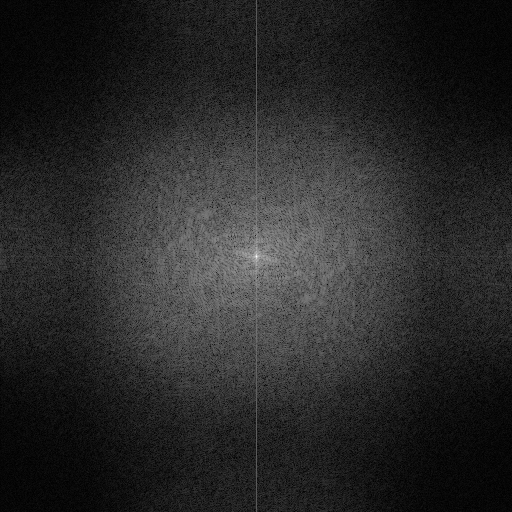
\includegraphics[width=0.32\textwidth]{spectre_tigre_log.png}
\caption{Module de la TFD du tigre, affiché avec $\log(1 + |F|)$.}
\label{fig:log}
\end{figure}

\subsection{Spectres des mires, de l'empreinte et de barbara}

On a fait nos prévisions avec la règle de l'énoncé : des rayures donnent deux points
symétriques, dans la direction perpendiculaire aux rayures, et d'autant plus loin du
centre que les rayures sont fines. On a mesuré la position des points en pixels à
partir du centre ; pour une sinusoïde, elle donne le nombre de périodes sur la taille
de l'image.

\begin{table}[H]
\centering
\caption{Spectres : prévision et observation (positions en pixels depuis le centre).}
\label{tab:spectres}
\begin{tabular}{|l|p{5.3cm}|p{6.2cm}|}
\hline
\textbf{Image} & \textbf{Prévision} & \textbf{Observation} \\
\hline
mire1 & deux points symétriques sur l'axe horizontal &
  points à $\pm 4$ sur l'axe horizontal : rayures verticales, 4 périodes sur la largeur \\
\hline
mire2 & même chose, plus loin du centre (rayures plus serrées) &
  points à $\pm 8$ sur l'axe horizontal : 8 périodes \\
\hline
mire3 & points hors des axes, par paires symétriques &
  deux paires : $(0, \pm 5)$ et $\pm(20, -10)$ (colonne, ligne), donc deux ondes
  superposées \\
\hline
fingerprint & un anneau centré & un anneau, plus une croix faible sur les axes \\
\hline
barbara & centre brillant, croix sur les axes, taches isolées dues aux rayures &
  conforme, avec des taches allongées dans des directions obliques \\
\hline
\end{tabular}
\end{table}

\begin{figure}[H]
\centering
\begin{tabular}{ccc}
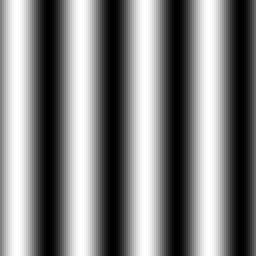
\includegraphics[width=0.27\textwidth]{mire1.png} &
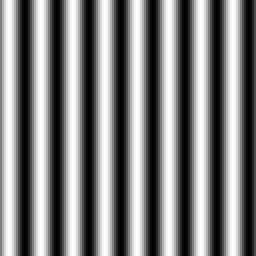
\includegraphics[width=0.27\textwidth]{mire2.png} &

\includegraphics[width=0.27\textwidth]{mire3.png} \\
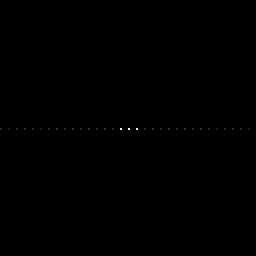
\includegraphics[width=0.27\textwidth]{spectre_mire1.png} &
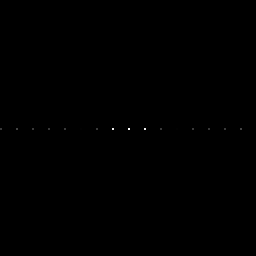
\includegraphics[width=0.27\textwidth]{spectre_mire2.png} &
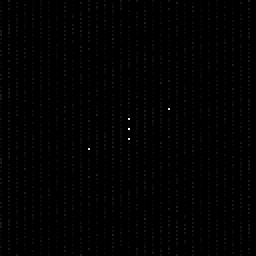
\includegraphics[width=0.27\textwidth]{spectre_mire3.png} \\
mire1 & mire2 & mire3
\end{tabular}
\caption{Mires ($128 \times 128$) et module de leur TFD (échelle logarithmique).}
\label{fig:mires}
\end{figure}

\begin{figure}[H]
\centering
\begin{tabular}{cc}
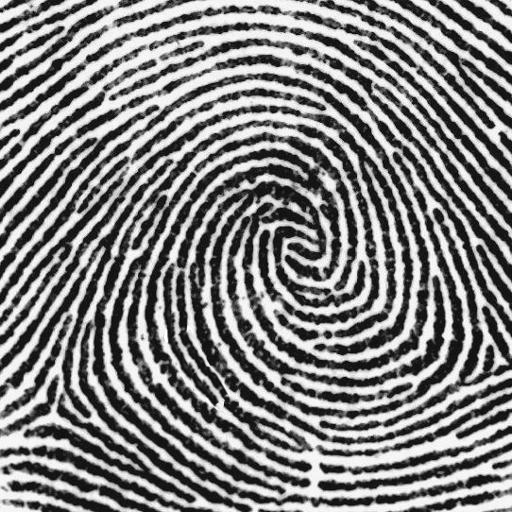
\includegraphics[width=0.36\textwidth]{fingerprint.png} &
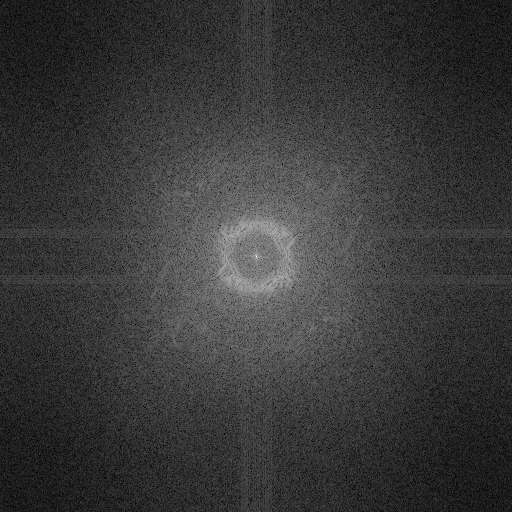
\includegraphics[width=0.36\textwidth]{spectre_fingerprint.png} \\
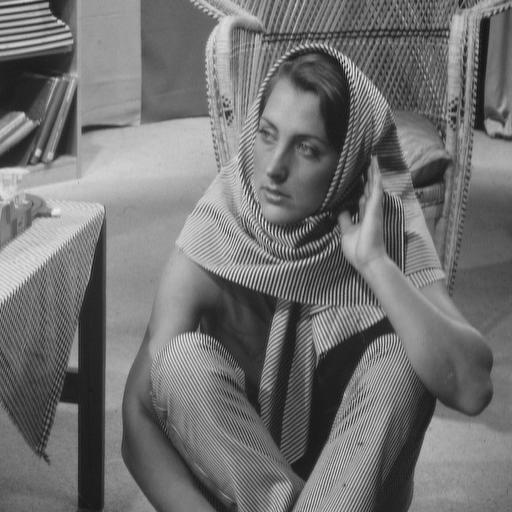
\includegraphics[width=0.36\textwidth]{barbara.png} &
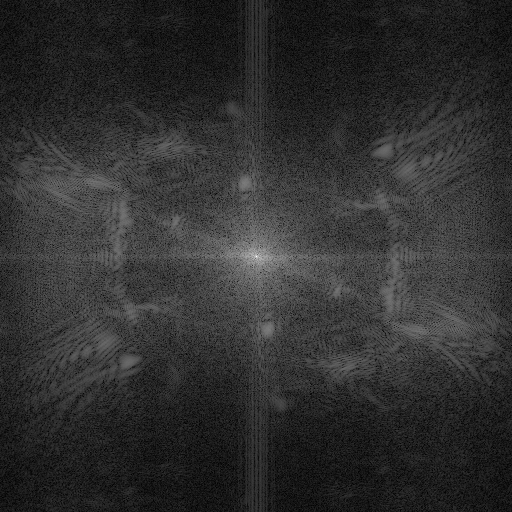
\includegraphics[width=0.36\textwidth]{spectre_barbara.png}
\end{tabular}
\caption{Empreinte et barbara ($512 \times 512$) avec le module de leur TFD.}
\label{fig:fp-barbara}
\end{figure}

Ce qu'on a observé :
\begin{itemize}
  \item \textbf{mire1, mire2.} 4 puis 8 périodes sur la largeur, donc des points à 4
        puis 8 pixels du centre. Par contre, on n'avait pas prévu la ligne de petits
        points sur l'axe horizontal, tous les 4 pixels (mire1) ou 8 pixels (mire2). On
        pense qu'elle vient de l'arrondi des pixels à des entiers : la mire n'est pas
        une sinusoïde exacte. Cette erreur est la même sur toutes les lignes de
        l'image, donc elle ne peut donner des points que sur l'axe horizontal, et elle
        se répète avec la période des rayures, donc tous les 4 (ou 8) pixels. Ces
        coefficients sont minuscules, on ne les voit que grâce au logarithme.
  \item \textbf{mire3.} Il y a deux paires de points, donc l'image est la somme de
        deux ondes : des rayures horizontales (5 périodes sur la hauteur)
        et des rayures obliques (point en $(20, -10)$, soit
        $\sqrt{20^2 + 10^2} \approx 22$ périodes).
  \item \textbf{Empreinte.} Les crêtes sont à peu près toutes espacées pareil mais
        tournent dans toutes les directions : un point par direction, à la même
        distance du centre, ce qui fait un anneau. Le fond gris vient des contours
        noir/blanc très nets (hautes fréquences).
  \item \textbf{Barbara.} Les taches loin du centre correspondent aux rayures du
        foulard, du pantalon et de la nappe, qui n'ont pas la même orientation.
  \item \textbf{Croix sur les axes.} On la voit pour l'empreinte, barbara et le tigre,
        pas pour les mires. Notre explication : la TFD traite l'image comme si elle se
        répétait, donc le bord droit touche le bord gauche ; sur une photo les deux
        bords sont différents, ce qui fait comme un contour vertical (et pareil en
        haut et en bas). Les mires ont un nombre entier de périodes, leurs bords se
        raccordent.
\end{itemize}

% =====================================================================
\section{Compression d'images}
% =====================================================================

\subsection{Annulation d'un seul coefficient}

On a annulé un coefficient de la TFD du tigre puis calculé la TFD inverse, en
repartant à chaque fois de la TFD complète. Pour chaque cas, on a mesuré l'écart
maximal entre l'image obtenue et l'originale.

\begin{table}[H]
\centering
\caption{Annulation d'un coefficient de la TFD du tigre ($n = 512$).}
\label{tab:ex4}
\begin{tabular}{|c|p{2.2cm}|p{4cm}|p{4.5cm}|}
\hline
\textbf{Coefficient} & \textbf{Écart max (niv. de gris)} & \textbf{Prévision} & \textbf{Observation} \\
\hline
$(n/2, n/2)$ & 84,4 &
  moyenne retirée ; zones proches de la moyenne noires & conforme
  (figure~\ref{fig:ex4}a) \\
\hline
$(n/2+1, n/2)$ & 20,2 &
  image quasi identique, léger dégradé & identique à l'\oe il ; écart : un dégradé
  vertical d'une période \\
\hline
$(n/2+100, n/2)$ & 0,16 & image inchangée & conforme ; écart : fines lignes
  horizontales \\
\hline
\end{tabular}
\end{table}

\begin{figure}[H]
\centering
\begin{subfigure}{0.3\textwidth}\centering
  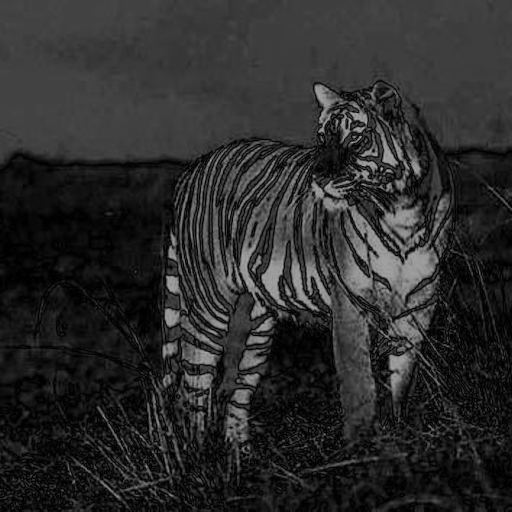
\includegraphics[width=\linewidth]{ex4_centre.png}
  \caption{centre annulé}
\end{subfigure}
\hfill
\begin{subfigure}{0.3\textwidth}\centering
  
\includegraphics[width=\linewidth]{ex4_diff_voisin.png}
  \caption{écart, $(n/2+1, n/2)$}
\end{subfigure}
\hfill
\begin{subfigure}{0.3\textwidth}\centering
  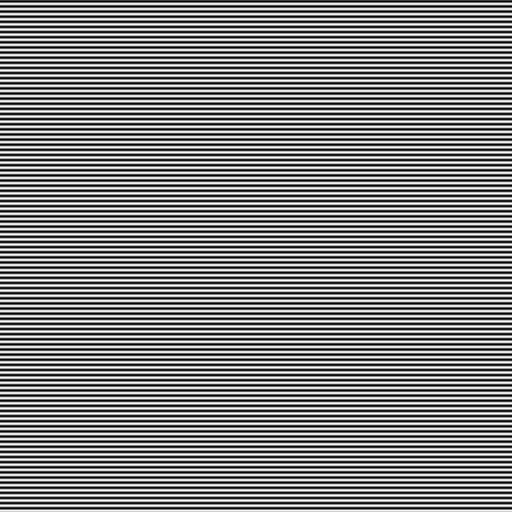
\includegraphics[width=\linewidth]{ex4_diff_HF.png}
  \caption{écart, $(n/2+100, n/2)$}
\end{subfigure}
\caption{Annulation d'un coefficient. Pour (b) et (c), l'image montre la différence
avec l'original, contraste étiré (gris moyen = 0).}
\label{fig:ex4}
\end{figure}

\begin{itemize}
  \item \textbf{Centre.} Comme prévu, on retire la moyenne : l'image vaut
        $I - 84{,}4$, avec des valeurs négatives. Comme on enregistre le module, on
        voit $|I - 84{,}4|$ : l'herbe, proche de la moyenne, devient noire, le ciel
        sombre devient gris, les rayures noires deviennent claires.
  \item \textbf{Voisin du centre.} L'écart est de 20 niveaux de gris, plus que ce
        qu'on pensait, mais on ne voit aucune différence : c'est un dégradé d'une seule
        période sur toute la hauteur (figure~\ref{fig:ex4}b), trop lent pour l'\oe il.
  \item \textbf{Haute fréquence.} 0,16 niveau de gris d'écart : invisible, comme
        prévu.
\end{itemize}
Le centre donne la luminosité moyenne, les coefficients proches les grandes
variations, ceux qui sont loin les détails fins, et ces derniers sont petits. C'est
ce qui permet de compresser.

\subsection{Compression par sélection des basses fréquences}

Dans notre fonction, les indices gardés vont de $n/2-k+1$ à $n/2+k$ ($2k$ valeurs) ;
le carré n'est donc pas tout à fait symétrique, mais ça ne change rien de visible.

\begin{table}[H]
\centering
\caption{Compression du tigre par un carré de côté $2k$ ($512^2 = 262\,144$
coefficients au total).}
\label{tab:ex5}
\begin{tabular}{|r|r|r|}
\hline
$k$ & \textbf{Coefficients gardés} & \textbf{Fraction} \\
\hline
4   & 64      & 0,024\,\% \\
\hline
8   & 256     & 0,098\,\% \\
\hline
16  & 1\,024  & 0,39\,\%  \\
\hline
32  & 4\,096  & 1,56\,\%  \\
\hline
64  & 16\,384 & 6,25\,\%  \\
\hline
128 & 65\,536 & 25\,\%    \\
\hline
\end{tabular}
\end{table}

\begin{figure}[H]
\centering
\begin{tabular}{ccc}
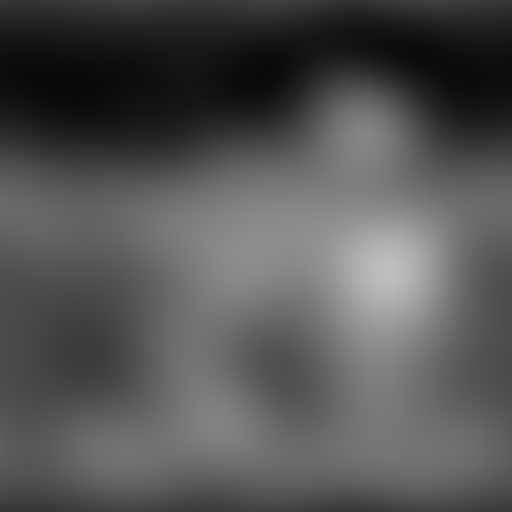
\includegraphics[width=0.3\textwidth]{ex5_k4.png} &
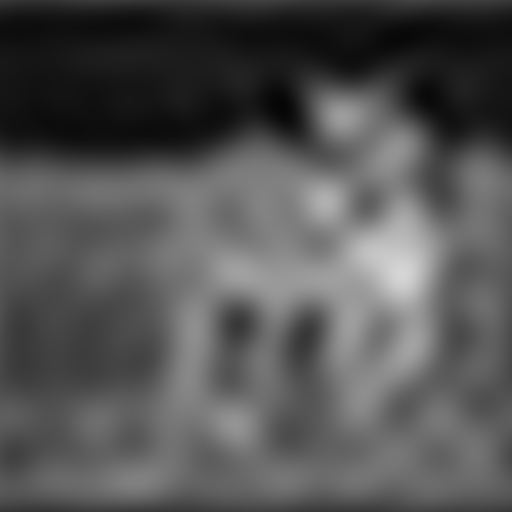
\includegraphics[width=0.3\textwidth]{ex5_k8.png} &
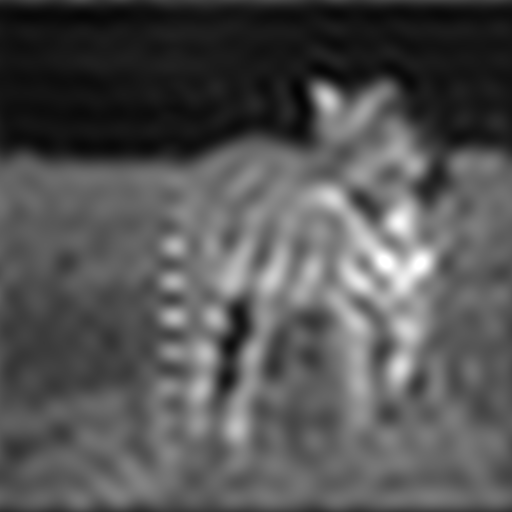
\includegraphics[width=0.3\textwidth]{ex5_k16.png} \\
$k = 4$ & $k = 8$ & $k = 16$ \\[0.2cm]
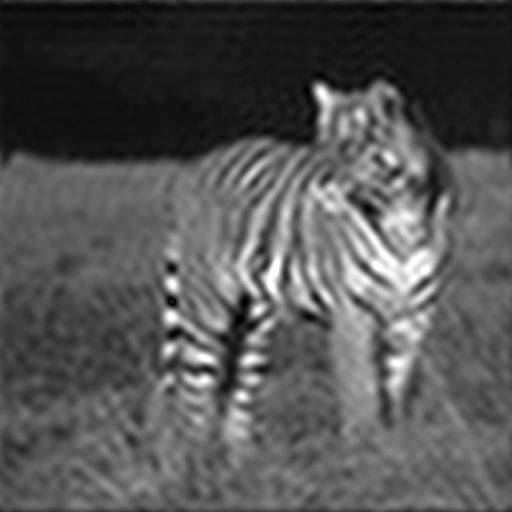
\includegraphics[width=0.3\textwidth]{ex5_k32.png} &
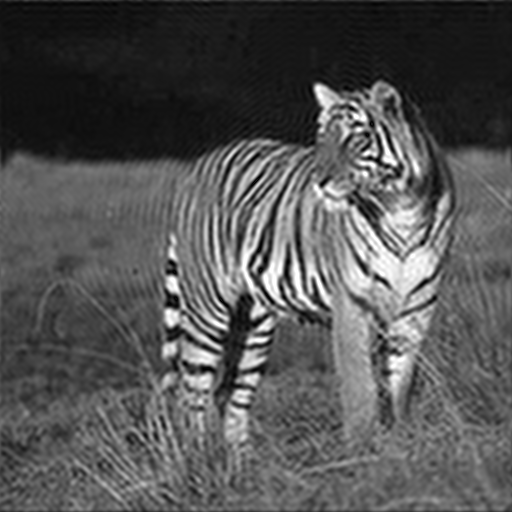
\includegraphics[width=0.3\textwidth]{ex5_k64.png} &
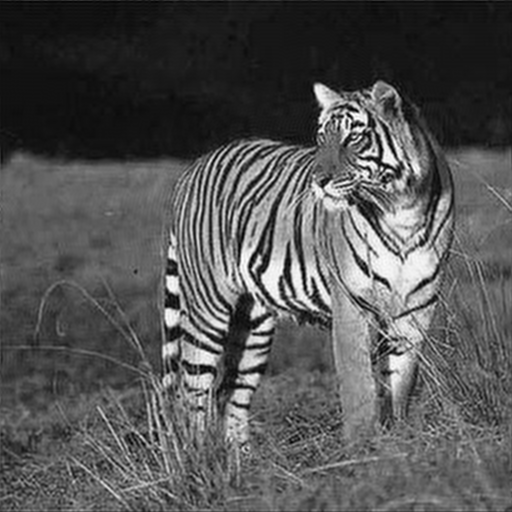
\includegraphics[width=0.3\textwidth]{ex5_k128.png} \\
$k = 32$ & $k = 64$ & $k = 128$
\end{tabular}
\caption{Tigre reconstruit à partir du carré de basses fréquences de côté $2k$.}
\label{fig:ex5}
\end{figure}

\begin{table}[H]
\centering
\caption{Compression par carré : prévision et observation.}
\label{tab:ex5prev}
\begin{tabular}{|c|p{6cm}|p{6cm}|}
\hline
$k$ & \textbf{Prévision} & \textbf{Observation} \\
\hline
4 & très floue, à peine reconnaissable & conforme : taches floues \\
\hline
16 & reconnaissable & conforme : silhouette et rayures floues \\
\hline
32 & floue, formes reconnaissables, oscillations près des contours &
  conforme : rayures nettes, herbe floue, ondulations près des contours \\
\hline
64 & visuellement bonne & conforme : seul le détail de l'herbe est perdu \\
\hline
128 & pas de différence nette & conforme : presque identique à l'original \\
\hline
\end{tabular}
\end{table}

Nos prévisions sont vérifiées. Le flou vient des hautes fréquences supprimées. Les
ondulations autour des contours (bien visibles à $k = 32$) sont le phénomène de
Gibbs : un contour net a besoin de toutes les fréquences, et on les coupe d'un coup à
$k$.

\subsection{Compression par seuillage}

On a testé notre fonction de seuillage sur le tigre avec un seuil de 30 : elle garde
30\,808 coefficients sur 262\,144, soit 11,8\,\%. Avec un seuil assez petit, on
garde donc déjà très peu de coefficients : la plupart sont petits. Ce test nous a
aussi donné l'ordre de grandeur du seuil pour l'exercice 7.

\subsection{\texorpdfstring{Comparaison des deux méthodes à 10\,\%}{Comparaison des deux méthodes à 10 \%}}

\paragraph{Ce qu'on a fait.} Pour le carré, on a pris $k = 81$, soit
$(2 \times 81)^2 = 26\,244$ coefficients (10,01\,\%). Pour le seuil, il fallait
trouver la valeur qui garde le même nombre de coefficients. Comme ce nombre diminue
quand le seuil augmente, on l'a cherché par dichotomie entre 0 et 200\,000 (le plus
grand coefficient ne peut pas dépasser $512 \times 255$), avec 40 itérations. À chaque
itération, on repart de la TFD complète, parce que notre fonction de seuillage modifie
le tableau. On a ensuite comparé les images, et calculé pour chaque méthode l'erreur
quadratique moyenne entre l'image $I$ et l'image reconstruite $I'$ :
\[
  \mathrm{MSE} = \frac{1}{n^2} \sum_{k,l} \bigl(I(k,l) - I'(k,l)\bigr)^2 .
\]

\begin{table}[H]
\centering
\caption{Comparaison carré / seuil, 26\,244 coefficients gardés (10\,\%).}
\label{tab:ex7}
\begin{tabular}{|l|l|r|r|r|}
\hline
\textbf{Image} & \textbf{Méthode} & \textbf{Gardés} & \textbf{Seuil} & \textbf{MSE (niv. de gris$^2$)} \\
\hline
tigre   & carré, $k = 81$ & 26\,244 & -     & 135,7 \\
\hline
tigre   & seuil           & 26\,244 & 35,6  & 74,0  \\
\hline
barbara & carré, $k = 81$ & 26\,244 & -     & 234,7 \\
\hline
barbara & seuil           & 26\,243 & 30,6  & 103,5 \\
\hline
\end{tabular}
\end{table}

\begin{figure}[H]
\centering
\begin{tabular}{ccc}
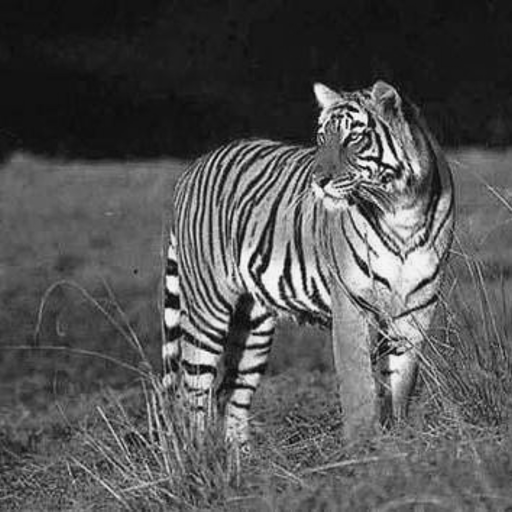
\includegraphics[width=0.3\textwidth]{tigre.png} &
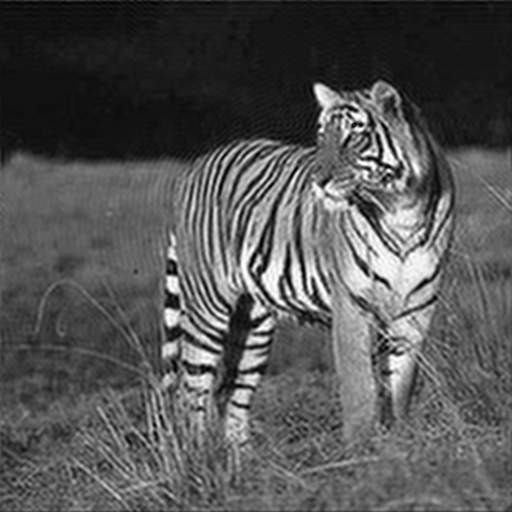
\includegraphics[width=0.3\textwidth]{ex7_tigre_carre.png} &
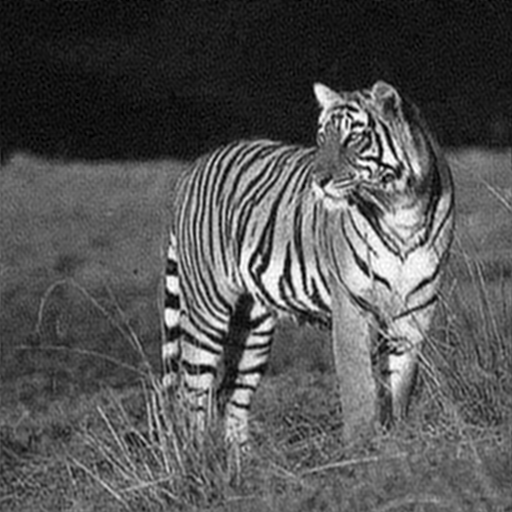
\includegraphics[width=0.3\textwidth]{ex7_tigre_seuil.png} \\
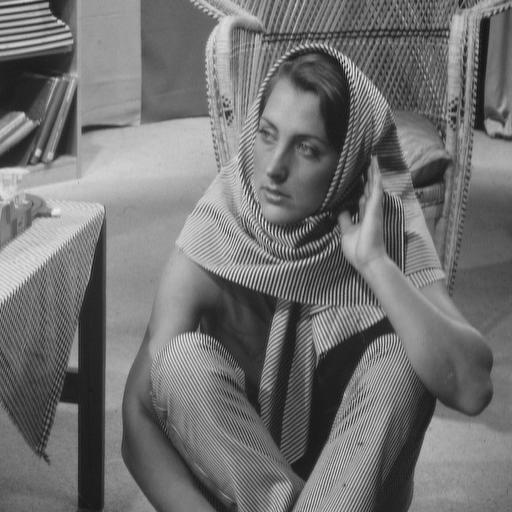
\includegraphics[width=0.3\textwidth]{barbara.png} &
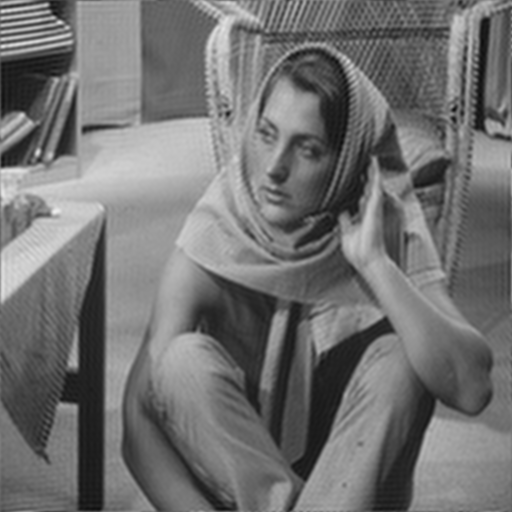
\includegraphics[width=0.3\textwidth]{ex7_barbara_carre.png} &
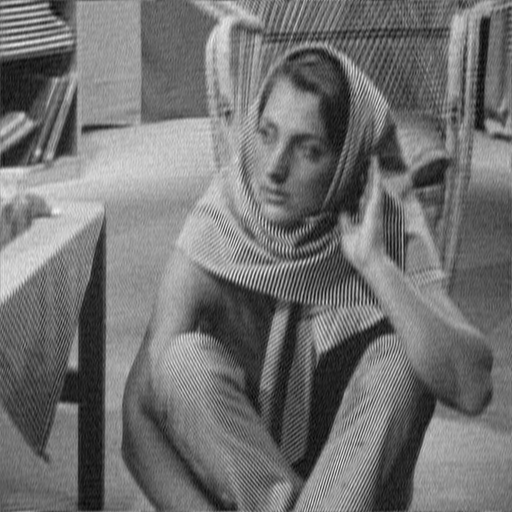
\includegraphics[width=0.3\textwidth]{ex7_barbara_seuil.png} \\
original & carré & seuil
\end{tabular}
\caption{Compression à 10\,\% des coefficients.}
\label{fig:ex7}
\end{figure}

\paragraph{Résultats.} Le seuil donne une MSE 1,8 fois plus faible pour le tigre et
2,3 fois pour barbara. Sur les images, le carré rend tout flou et efface les rayures
du pantalon et du foulard de barbara. Le seuil garde ces rayures, mais on voit un
léger grain dans les zones lisses.

\paragraph{Pourquoi le seuil est meilleur.} Avec le $1/n$, la TFD 2D conserve
l'énergie (Parseval), donc l'erreur vaut
\[
  \mathrm{MSE} = \frac{1}{n^2} \sum_{\text{coefficients annulés}} |F(u,v)|^2 .
\]
Pour un nombre de coefficients gardés fixé, cette somme est la plus petite
quand on annule les plus petits modules, et c'est exactement ce que fait le seuil.

L'écart est plus grand pour barbara : ses rayures sont des hautes fréquences avec un
grand module (les taches loin du centre de son spectre). Le carré les supprime, le
seuil les garde.

\paragraph{Limite.} Avec le carré, on sait où sont les coefficients gardés (il suffit
de $k$). Avec le seuil, il faudrait aussi stocker la position de chacun, donc à nombre
de coefficients égal, le fichier serait plus gros. La comparaison à 10\,\% des
coefficients avantage donc un peu le seuil.

% =====================================================================
\section{Conclusion}
% =====================================================================

Notre FFT et son inverse donnent les bons résultats, et la multiplication par FFT
donne les mêmes coefficients que la méthode classique. Les mesures confirment les
complexités : quand $n$ double, le temps est multiplié par environ 4 pour la méthode
par les coefficients et par un peu plus de 2 pour la FFT. À cause de sa constante
45 fois plus grande, la FFT n'est plus rapide qu'à partir de quelques centaines de
coefficients ; après, le gain grandit comme $n / \ln n$.

En 1D comme en 2D, nos prévisions sur les spectres ont été vérifiées ; les détails
qu'on n'avait pas prévus (petits points des mires, deux ondes dans mire3) ont une
explication. Les coefficients loin du centre sont petits et ne changent presque rien
à l'image, ce qui permet de compresser. Le carré de basses fréquences donne une image
reconnaissable avec moins de 1\,\% des coefficients, mais floue. À 10\,\% des
coefficients, le seuillage donne une erreur 1,8 à 2,3 fois plus faible, ce qu'on
explique avec Parseval, surtout sur une image avec beaucoup de textures comme
barbara. Son inconvénient est qu'il faut stocker la position des coefficients
gardés.

\end{document}
